\documentclass[../thesis.tex]{subfiles}
\begin{document}
\chapter{Applied Integrated Lifetimes}

\section{CBP Host Thickness}

\begin{figure}[ht]
\centering
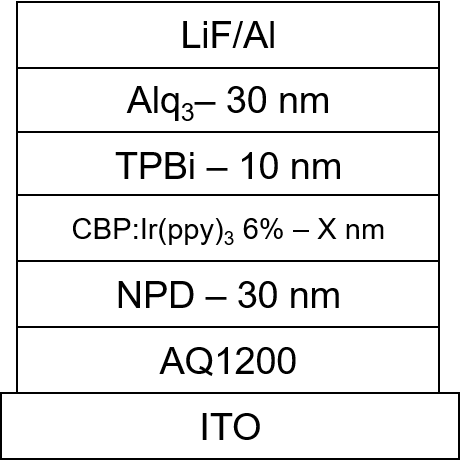
\includegraphics[width=0.48\textwidth]{lifetimeApplications/architecture}
\caption{Device architecture, featuring EML thicknesses of X=10,20, and 30 nm}
\label{fig:architecture}
\end{figure}

\begin{figure}[ht]
\centering
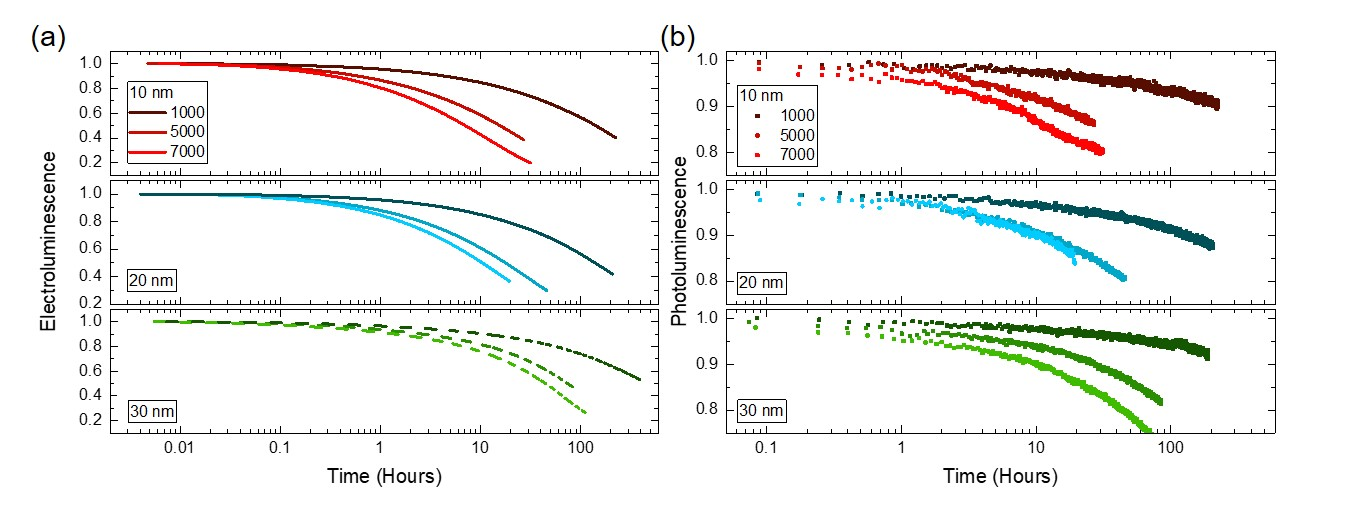
\includegraphics[width=0.48\textwidth]{lifetimeApplications/elpl}
\caption{Device decay curves for multiple values of the initial luminance as a function of emissive layer thickness.  Loss in (a) electroluminescence (EL) and (b) photoluminescence (PL) are shown and decrease monotonically with increasing luminance.  For devices with a 10-nm-thick emissive layer, initial luminance values are 1000 $cd/m^2$, 5000 $cd/m^2$, and 7000 $cd/m^2$.  For devices with a 20-nm- or 30-nm-thick emissive layer, initial luminance values are 1000 $cd/m^2$, 5000 $cd/m^2$, and 7100 $cd/m^2$. }
\label{fig:elpl}
\end{figure}

\begin{figure}[ht]
\centering
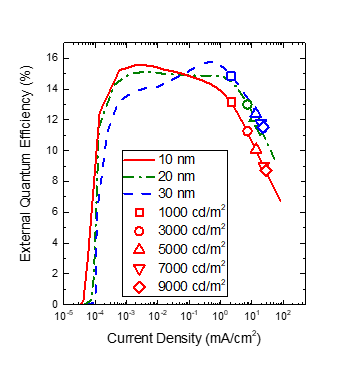
\includegraphics[width=0.48\textwidth]{lifetimeApplications/eqe}
\caption{External Quantum Efficiency ($\eta_{EQE}$) for the three architectures.  Operational points for lifetime are shown in symbols.}
\label{fig:eqe}
\end{figure}


\begin{table}[h]
\centering
\begin{tabular}{c|c|c|c|c}
$d_{EML}$ (nm) & $L_0$ (cd/m$^2$) & $J$ (mA/cm$^2$) & $V_0$ (V) & $t_{50}$ (hours) \\
\hline
& 1000 & 2.2 & 4.2 & 139.0 \\
& 3000 & 7.2 & 5.1 & 39.9 \\
10 & 5000 & 13.6 & 5.4 & 15.8 \\
& 7000 & 14.4 & 6.2 & 6.9 \\
& 9000 & 28.0 &  6.3 & 5.3 \\
\hline
& 1000 & 2.2 & 5.4 & 141.1 \\
& 3000 & 7.2 & 6.0 & 33.1 \\
20 & 5000 & 12.4 & 7.2 & 17.2 \\
& 7100 & 19.2 & 7.3 & 10.0 \\
& 9000 & 24.0 &  7.5 & 8.0 \\
\hline
& 1000 & 2.2 & 5.9 & 474 \\
30 & 5000 & 13.6 & 7.3 & 74.4\\
& 7100 & 19.6 & 7.6 & 46 \\
& 8000 & 22.4 &  7.7 & 38.1 \\

\end{tabular}
\caption{Summary of device lifetimes.  For each device, the starting luminance ($L_0$), current density ($J$), starting voltage ($V_0$) and time at which 50\% of the initial luminance is reached ($t_{50}$) are reported.}
\label{tab:lifetime_summary}
\end{table}

\begin{figure}[ht]
\centering
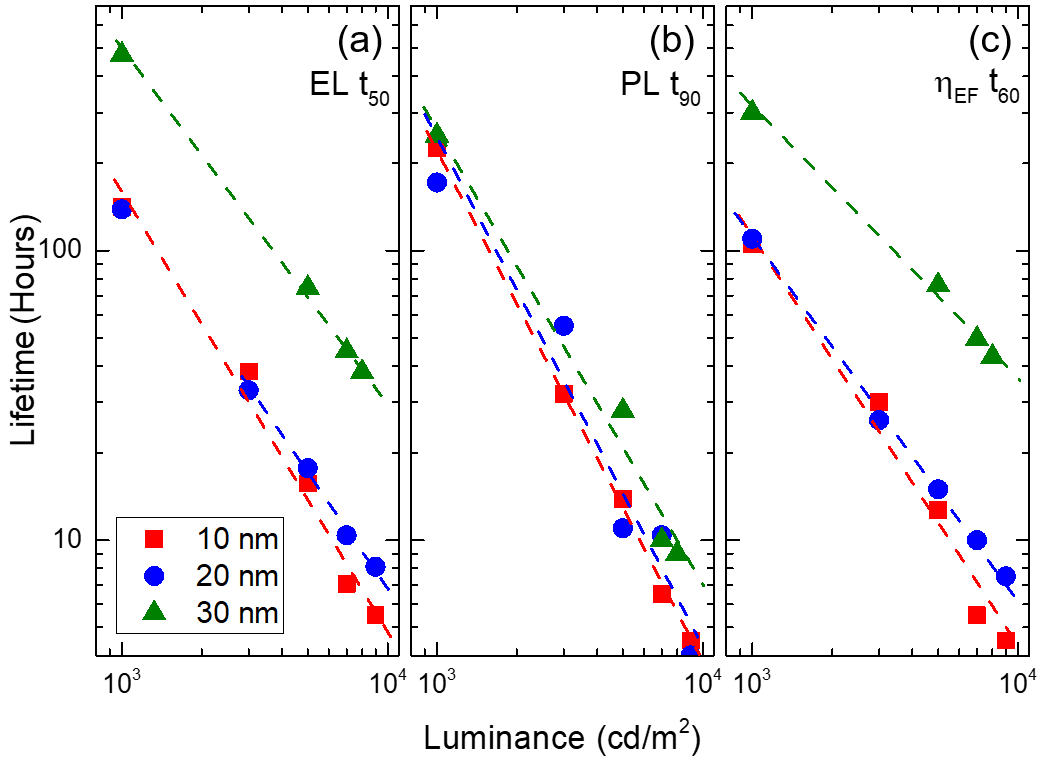
\includegraphics[width=0.48\textwidth]{lifetimeApplications/tx_components}
\caption{Extracted lifetimes for all 3 architecures as a function of luminance.}
\label{fig:tx_components}
\end{figure}

\section{MEML Luminance Scaling}


\section{Dow Cohost}



\ifcsdef{mainfile}{}{\bibliography{../library}}
\end{document}
